\documentclass[12pt,a4paper]{article}
% \usepackage{ctex}
\usepackage{amsmath,amscd,amsbsy,amssymb,latexsym,url,bm,amsthm}
\usepackage{epsfig,graphicx,subfigure}
\usepackage{enumitem,balance}
\usepackage{wrapfig}
\usepackage{mathrsfs,euscript}
\usepackage[usenames]{xcolor}
\usepackage{hyperref}
\usepackage[vlined,ruled,linesnumbered]{algorithm2e}
\usepackage{array}
\hypersetup{colorlinks=true,linkcolor=black}

\newtheorem{theorem}{Theorem}
\newtheorem{lemma}[theorem]{Lemma}
\newtheorem{proposition}[theorem]{Proposition}
\newtheorem{corollary}[theorem]{Corollary}
\newtheorem{exercise}{Exercise}
\newtheorem*{solution}{Solution}
\newtheorem{definition}{Definition}
\theoremstyle{definition}

\renewcommand{\thefootnote}{\fnsymbol{footnote}}

\newcommand{\postscript}[2]
 {\setlength{\epsfxsize}{#2\hsize}
  \centerline{\epsfbox{#1}}}

\renewcommand{\baselinestretch}{1.0}

\setlength{\oddsidemargin}{-0.365in}
\setlength{\evensidemargin}{-0.365in}
\setlength{\topmargin}{-0.3in}
\setlength{\headheight}{0in}
\setlength{\headsep}{0in}
\setlength{\textheight}{10.1in}
\setlength{\textwidth}{7in}
\makeatletter \renewenvironment{proof}[1][Proof] {\par\pushQED{\qed}\normalfont\topsep6\p@\@plus6\p@\relax\trivlist\item[\hskip\labelsep\bfseries#1\@addpunct{.}]\ignorespaces}{\popQED\endtrivlist\@endpefalse} \makeatother
\makeatletter
\renewenvironment{solution}[1][Solution] {\par\pushQED{\qed}\normalfont\topsep6\p@\@plus6\p@\relax\trivlist\item[\hskip\labelsep\bfseries#1\@addpunct{.}]\ignorespaces}{\popQED\endtrivlist\@endpefalse} \makeatother

\begin{document}
\noindent

%========================================================================
\noindent\framebox[\linewidth]{\shortstack[c]{
\Large{\textbf{Lab09-Network Flow}}\vspace{1mm}\\
CS214-Algorithm and Complexity, Xiaofeng Gao \& Lei Wang, Spring 2021.}}
\begin{center}
\footnotesize{\color{red}$*$ If there is any problem, please contact TA Yihao Xie. }

\footnotesize{\color{blue}$*$ Name: Wendi Chen  \quad Student ID: 519021910071 \quad Email: chenwendi-andy@sjtu.edu.cn}
\end{center}

\begin{enumerate}
    \item  Consider there is a network consists $n$ computers. For some pairs of computers, a wire $i$ exists in the pair, which means these two computers can communicate with each other. When a signal passes through the wires, the noise in the signal will be amplified. If you know the magnification rate of noise $m_{i,j}$ of each wire (which must be greater than 1). Design an algorithm to find the route  for each other computer to send signals to the computer $v$ with the minimum total magnification rate of noise and analyze the time complexity.
    
    \begin{solution}
    ~\\
    This problem is similar to the \emph{Single-Source Shortest Paths} problem. What is different is that this time we multiply the weights of all edges on one path instead of calculating the sum of them. Also, because the magnification rate of noise (MRN) $m_{i,j}$ of each wire is greater than 1, the total MRN is always increasing when we add a new edge to the route. All the properties imply that we can use \emph{Dijkstra's Algorithm} to solve this problem.\\
    We abstract the computer network to be a undirected graph $G = (V,E)$ with edge-weight function $m:E\to R$. The weight of path $P = v_1\to \dots \to v_k$ is defined to be
    \begin{equation*}
        m(P) = \Pi_{i=1}^{k-1}m(v_i,v_{i+1})
    \end{equation*}
    Thus, we just want to find a shortest path $u$ to $v$ for every $u \in V$. Now, we use the \emph{Dijkstra's Algorithm} with binary heap to solve this problem. (Alg.\ref{Alg-route})
    
    \begin{minipage}[t]{0.9\textwidth}
        \begin{algorithm}[H]
        \KwIn{$G=(V,E)$ is a connected, undirected graph;$v\in V$}
        \KwOut{An array $path(u)$ which indicates the next vertex on the path from $u$ to $v$}
        
        \BlankLine
        \caption{Algorithm to Find the Route with the Minimum MRN in a Computer Network}
        \label{Alg-route}
        $path[v_1,\dots,v_n]\leftarrow -1$\;
        $d[v_1,\dots,v_n]\leftarrow +\infty$\;
        $d[v]\leftarrow 0$\;
        $\text{priority-queue } Q\leftarrow \emptyset$\;
        $S\leftarrow\emptyset$\;
        \For{$u\in V$ }{
            $INSERT(Q,u)$\;
        }
        \While{$Q\neq\emptyset$}{
            $u\leftarrow EXTRACT-MIN(Q)$\;
            $S\leftarrow S\cup\{u\}$\;
            \For{$v^{'}\in Adj[u]$}{
            \If{$d[v^{'}]>d[u]\times w(u,v^{'})$}{
                $path[v^{'}]\leftarrow u$\;
                $d[v^{'}]\leftarrow d[u]\times w(u,v^{'})$\;
                $UPDATE-KEY(Q,v^{'})$\;
                }
            }
        }
        \end{algorithm}
    \end{minipage}
    
    The time complexity of \emph{EXTRACT-MIN}, \emph{INSERT} and \emph{UPDATE-KEY} is $O(\log(|V|)$. Thus, the whole time complexity is $O((|V|+|E|)\log(|V|)$.
    \end{solution}
	
	\item Suppose that we wish to maintain the transitive closure of a directed graph $G=(V,E)$ as we insert edges into $E$. That is, after each edge has been inserted, we want to update the transitive closure of the edges inserted so far. Assume that the graph $G$ has no edges initially and that we represent the transitive closure as a boolean matrix.
	\begin{enumerate}
	    \item Show how to update the transitive closure of a graph $G=(V,E)$ in $O(V^2)$ time when a new edge is added to $G$.
	    \item Give an example of a graph $G$ and an edge $e$ such that $\Omega(V^2)$ time is required to update the transitive closure after the insertion of $e$ into $G$, no matter what algorithm is used.
	    \item Describe an efficient algorithm for updating the transitive closure as edges are inserted into the graph. For any sequence of $m$ insertions, your algorithm should run in total time $\sum_{i=1}^m t_i=O(V^3)$, where $t_i$ is the time to update the transitive closure upon inserting the $i$th edge. Prove that your algorithm attains this time bound.
	\end{enumerate}
	\begin{solution}
	~
	\begin{enumerate}
	    \item 
	    Assume that we add a new edge $(v_p,v_q)$. In order to update the transitive closure, we have to check every pair of vertices $(v_i,v_j)$. If there is a path from $v_i$ to $v_p$ and another path from $v_q$ to $v_j$, we can add $(v_i,v_j)$ to the transitive closure. We set that $n=|V|$.
	    
	    \begin{minipage}[t]{0.85\textwidth}
        \begin{algorithm}[H]
        \KwIn{The original transitive closure $T$ (a $n\times n$ matrix) of a directed graph $G=(V,E)$; a new edge $e=(v_p,v_q)$ with $v_p,v_q\in E$}
        \KwOut{The new transitive closure $T^{'}$ after adding $e$ to $G$} 
        
        \BlankLine
        \caption{Algorithm to Update a Transitive Closure}
        \label{Alg-closure}
        \For{$i\leftarrow1 \text{ to } n$ }{
            \For{$j\leftarrow 1 \text{ to } n$}{
                \If{$T[i][p]=1\text{ and }T[q][j]=1$}{
                    $T[i][j]\leftarrow1$\;
                }
            }
        }
            \end{algorithm}
        \end{minipage}
    
    From Alg.\ref{Alg-closure}, we can find that the time complexity is $O(n^2)=O(V^2)$.
    
    \item
    The graph $G$ is composed of two strongly connected components with $\frac{|V|}{2}$ vertices respectively and there is no edge between them. Let $e$ be an edge that connects the two SCCs. The example when $|V|=6$ is given in Figure.\ref{Fig-closure}.
    \begin{figure}[!htbp]
    	\centering
    	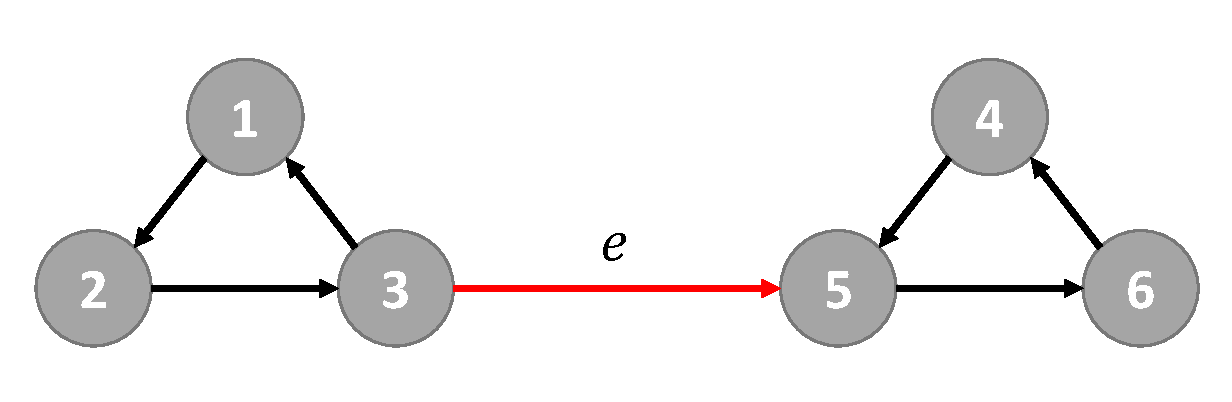
\includegraphics[width=0.7\textwidth]{Fig-closure.pdf}
    	\caption{An example graph when $|V|=6$}
    	\label{Fig-closure}
    \end{figure}
    
    The matrix of the original transitive closure has the following format.
    
     \begin{equation*}
     \left[
     \begin{array}{cccccc}
         1 & \dots & 1 & 0 & \dots & 0 \\
         \vdots & \ddots & \vdots & \vdots & \ddots & \vdots \\
         1 & \dots & 1 & 0 & \dots & 0 \\ 
         0 & \dots & 0 & 1 & \dots & 1 \\
         \vdots & \ddots & \vdots & \vdots & \ddots & \vdots \\
         0 & \dots & 0 & 1 & \dots & 1
     \end{array}
     \right]        
     \end{equation*}
    
    If we add the new edge $e$, the matrix of the transitive closure will be like
    
     \begin{equation*}
     \left[
     \begin{array}{cccccc}
         1 & \dots & 1 & 1 & \dots & 1 \\
         \vdots & \ddots & \vdots & \vdots & \ddots & \vdots \\
         1 & \dots & 1 & 1 & \dots & 1 \\ 
         0 & \dots & 0 & 1 & \dots & 1 \\
         \vdots & \ddots & \vdots & \vdots & \ddots & \vdots \\
         0 & \dots & 0 & 1 & \dots & 1
     \end{array}
     \right]        
     \end{equation*}
    
    That means we have to update the value of $\frac{|V|^2}{4}$ elements in the matrix. Thus, no matter what algorithm is used, $\Omega(V^2)$ time is required to update the transitive closure. 
    
    \item
    In fact, in problem (a), we check each possible route too many times that we may have done some useless work. For example, if $T[i][q]$ is already 1, the new edge will not create any new route from $i$ to $j$. Thus, we can revise Alg.\ref{Alg-closure} to a new one (Alg.\ref{Alg-newclosure}).
    
    \begin{minipage}[t]{0.85\textwidth}
        \begin{algorithm}[H]
        \KwIn{The original transitive closure $T$ (a $n\times n$ matrix) of a directed graph $G=(V,E)$; a new edge $e=(v_p,v_q)$ with $v_p,v_q\in E$}
        \KwOut{The new transitive closure $T^{'}$ after adding $e$ to $G$} 
        
        \BlankLine
        \caption{A Better Algorithm to Update a Transitive Closure}
        \label{Alg-newclosure}
        \For{$i\leftarrow1 \text{ to } n$ }{
            \If{$T[i][q]=0\text{ and }T[i][p]=1$}{
                \For{$j\leftarrow 1 \text{ to } n$}{
                    \If{$T[q][j]=1$}{
                        $T[i][j]\leftarrow1$\;
                    }
                }
            }
        }
        \end{algorithm}
        \end{minipage}
    
        Let us analyze the time complexity. \\
        We analyze the last three lines first. We assert that during the whole process of inserting, this part can be executed $O(V^2)$ times. That is because they're executed only when $T[i][q]=0$ and after the execution $T[i][q]$ are set to be 1. The last three lines have a time complexity of $O(V)$. Then, they totally cost $O(V^3)$.\\
        For the rest part, we can add at most $V^2$ edges and the outer loop cost $O(V)$. Thus, the rest part has a time complexity of $O(V^3)$.\\
        Therefore, the overall time complexity is $O(V^3)$.
	\end{enumerate}
	\end{solution}
	
	\item An $n\times n$ grid is an undirected graph consisting of n rows and n columns of vertices, as shown in Figure 26.11. We denote the vertex in the $i$th row and the $j$th column by $(i,j)$. All vertices in a grid have exactly four neighbors, except for the boundary vertices, which are the points $(i,j)$ for which $i = 1, i = n, j = 1$, or $j = n$.
    Given $m\leqslant n^2$ starting points $(x_1,y_1), (x_2, y_2), ... , (x_m, y_m)$ in the grid, the escape problem is to determine whether or not there are $m$ vertex-disjoint paths from the starting points to any $m$ different points on the boundary such that every vertex in $V$ is included in at most one of the $m$ paths. For example, the grid in Figure \ref{Fig-EscapeProblem}(a) has an escape, but the grid in \ref{Fig-EscapeProblem}(b) does not.
    \begin{figure}[!htbp]
	\centering
	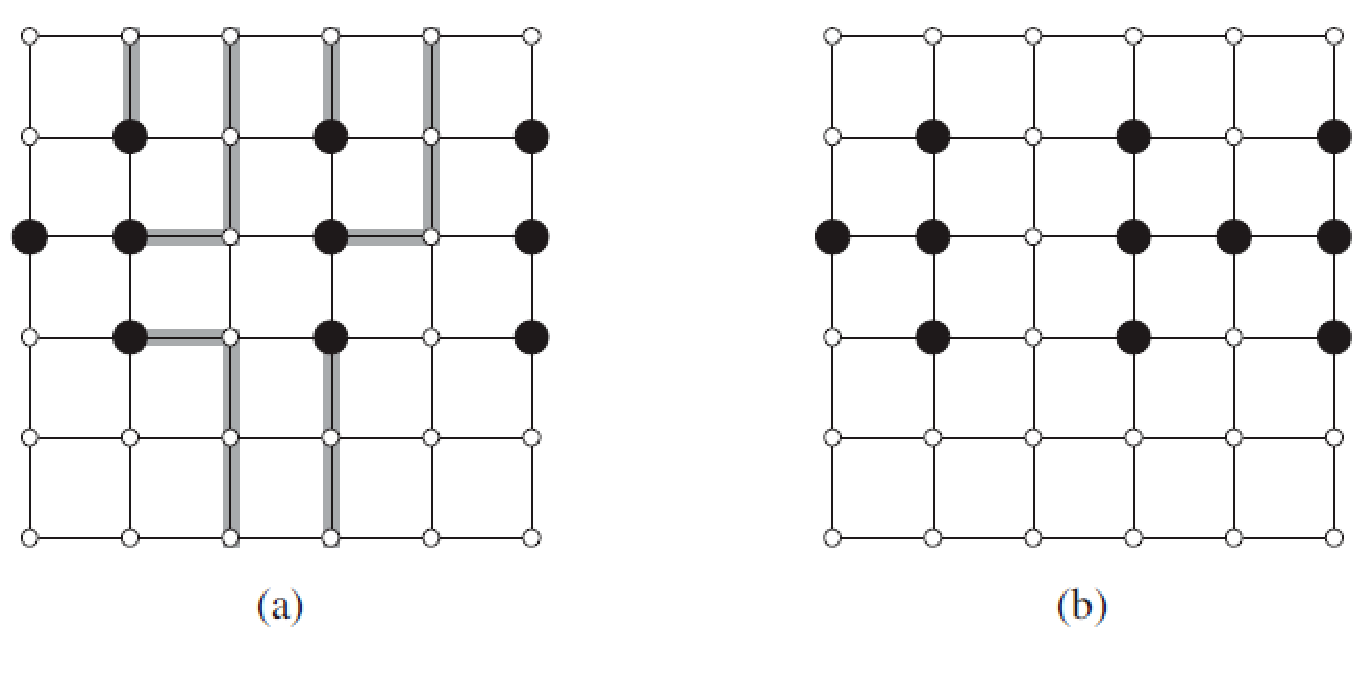
\includegraphics[width=0.5\textwidth]{Fig-EscapeProblem.pdf}
	\caption{Grids for the escape problem. Starting points are black, and other grid vertices are white. (a) A grid with an escape, shown by shaded paths. (b) A grid with no escape.}
	\label{Fig-EscapeProblem}
	\end{figure}
    \begin{enumerate}
        \item Consider a flow network in which vertices, as well as edges, have capacities. That is, the total positive flow entering any given vertex is subject to a capacity constraint. Show that determining the maximum flow in a network with edge and vertex capacities can be reduced to an ordinary maximum-flow problem on a flow network of comparable size. That is, the sizes of the two graph are in the same order of magnitude.
        \item Describe an efficient algorithm to solve the escape problem, and analyze its running time.
    \end{enumerate}
    
    \begin{solution}
    ~
    \begin{enumerate}
        \item 
        Let $G=(V,E)$ be the original flow network whose vertices and edges have capacities. To complete the transformation, we can do the following replacement. For every vertex $v\in V$ with capacity $c(v)$, we replace it with $v_1$ and $v_2$ and $c(v_1,v_2) = c(v)$. For every edge $(u_i,v)$, we replace it with $(u_i,v_1)$, and for every edge $(v,u_j)$, we replace it with $(v_2,u_j)$. And we have the equation $c(u_i,v_1)=c(u_i,v)$ and $c(v,u_j)=c(v_2,u_j)$. After these operations, we get an ordinary flow network $G^{'}=(V^{'},E^{'})$, where $|V^{'}| = 2|V|$ and $|E^{'}|=|E|+|V|$. Because we have $|V|=O(|E|)$, the new flow network has the same order of magnitude as the old one.
        \item
        First, we transform the grid into a flow network in which vertices and edges have capacities. We replace all edges between adjacent edges with two opposite directed edges whose capacities are one (it can be proved that only one of two edges will be used). For all vertices, we give them a capacity of one. At last, we set a source $s$ and a sink $t$ with no capacity limits. For every starting points, there is a directed edge with capacity of one from $s$ to it. For every boundary vertex, there is a directed edge with capacity of one from it to $t$.\\
        Next, we transform the network to an ordinary flow network according to (a).\\
        At last, we can solve this problem by transforming it into a maximum flow problem. We can use \emph{Ford-Fulkerson} algorithm to solve it. If the maximum flow equals $m$, we can say the grid has an escape. Otherwise, it has no escape.\\
        Now, let us analyze the time complexity. The transformation process has a time complexity of $O(n^2)$. Because the two network has the same order of magnitude. The \emph{Ford-Fulkerson} algorithm has a time complexity of $O(C n^4)$ and here we have $C=1$. Thus, the overall time complexity is $O(n^4)$.
    \end{enumerate}
    \end{solution}
\end{enumerate}

\textbf{Remark:} Please include your .pdf, .tex files for uploading with standard file names.
\newpage


%========================================================================
\end{document}